\section{Rechnungswesen mit SAP ERP Financials}
\subsection{Komponenten}
\label{sec:Komponenten}
Das Ziel von ERP-Systemen (Enterprise Resource Planning\abk{ERP}{Enterprise Resource Planning}) ist die Erfassung aller wesentlichen betrieblichen Abläufe zur Planung, Dokumentation und Steuerung. Die ERP-Software der Firma SAP ist eine branchenübergreifende Standardlösung, die sich an unterschiedlichste Anforderungen verschiedener Unternehmen anpassen lässt (Customizing\abk{Customizing}{Softwareanpassung an betriebs- und branchenspezifische Vorgaben}). Die Anwendungen erlauben eine ganzheitliche Abwicklung von abteilungs- und\\bereichsübergreifenden Prozessen der organisatorischen Einheit. Die Struktur von SAP ERP orientiert sich an den klassischen betriebswirtschaftlichen Funktionen eines Unternehmens. Auf der obersten Ebene finden sich die funktionalen Sichten\footnote{Vgl. \cite{Bauer2009}, S. 78 f.}:
\begin{compactitem}
\item Finanzen
\item Personalwirtschaft
\item Beschaffung und Logistik
\item Produktion
\item Vertrieb
\end{compactitem}
Diese Struktur wird weiter in Module, Komponenten, Unterkomponenten und Transaktionen aufgeteilt. Während die Firma SAP für die Module und Komponenten des bereits 1992 erschienenen SAP R/3 noch klare Bezeichnungen etabliert hat, verzichtet sie im heutigen Marketing der Weiterentwicklung SAP ERP darauf\footnote{Vgl. \cite{Klein2010}, S. 9 f.}\footnote{Vgl. \cite{Hefner2001}, S. 25}. Für eine exakte Einordnung im Themenkomplex, werden in dieser Arbeit auch die Modul- und Komponentenbezeichnungen beigefügt.

SAP ERP Financials als Teil von SAP ERP ist die Anwendung für die Unternehmenssicht Finanzen, welche folgende Module beinhaltet\footnote{Vgl. \cite{Hefner2001}, S. 27}\footnote{Vgl. \cite{Muir2009}, S. 72 ff.}
\begin{compactitem}
\item Financial Accounting (Finanzwesen -- FI)
\item Management Accounting (Controlling -- CO)
\item Enterprise Controlling (Unternehmenscontrolling -- EC)
\item Treasury (TR)
\item Investment Management (IM)
\end{compactitem}
Diese Arbeit konzentriert sich auf das Rechnungswesen (FI, CO) mit SAP ERP Financials, welches in den Modulen Financial Accounting (FI) und Management Accounting (CO) abgebildet und in den folgenden Kapiteln näher behandelt wird\footnote{Vgl. \cite{Patel2009}, S. 23}.

\subsection{Konzernstruktur}
Bei der Einführung eines SAP ERP-Systems müssen die betrieblichen Organisationsstrukturen, die sich aus unterschiedlichen Gesellschaften und operativen Einheiten eines Konzerns zusammensetzt, in diesem abgebildet werden\footnote{Vgl. \cite{Jacob2008}, S. 8}.
Jedes Modul des SAP ERP Systems hat ihre eigenen Organisationsstrukturen\footnote{Vgl. \cite{Klein2010}, S. 98}. Im Folgenden werden die Organisationseinheiten des internen und externen Rechnungswesens beschrieben. Abbildung~\ref{abb2} auf Seite \pageref{abb2} zeigt ein Beispiel einer Konzernstruktur im SAP Rechnungswesen.

Der Mandant stellt die oberste Konzernhierarchieebene dar und bildet ein Konzernunternehmen mit allen zugehörigen Gesellschaften ab, deren Ergebnisse in das Konzernergebnis einfließen. Gesellschaftsübergreifende Daten und Parameter werden auf Mandantenebene abgelegt.
\begin{figure}[htbp]
\begin{center}
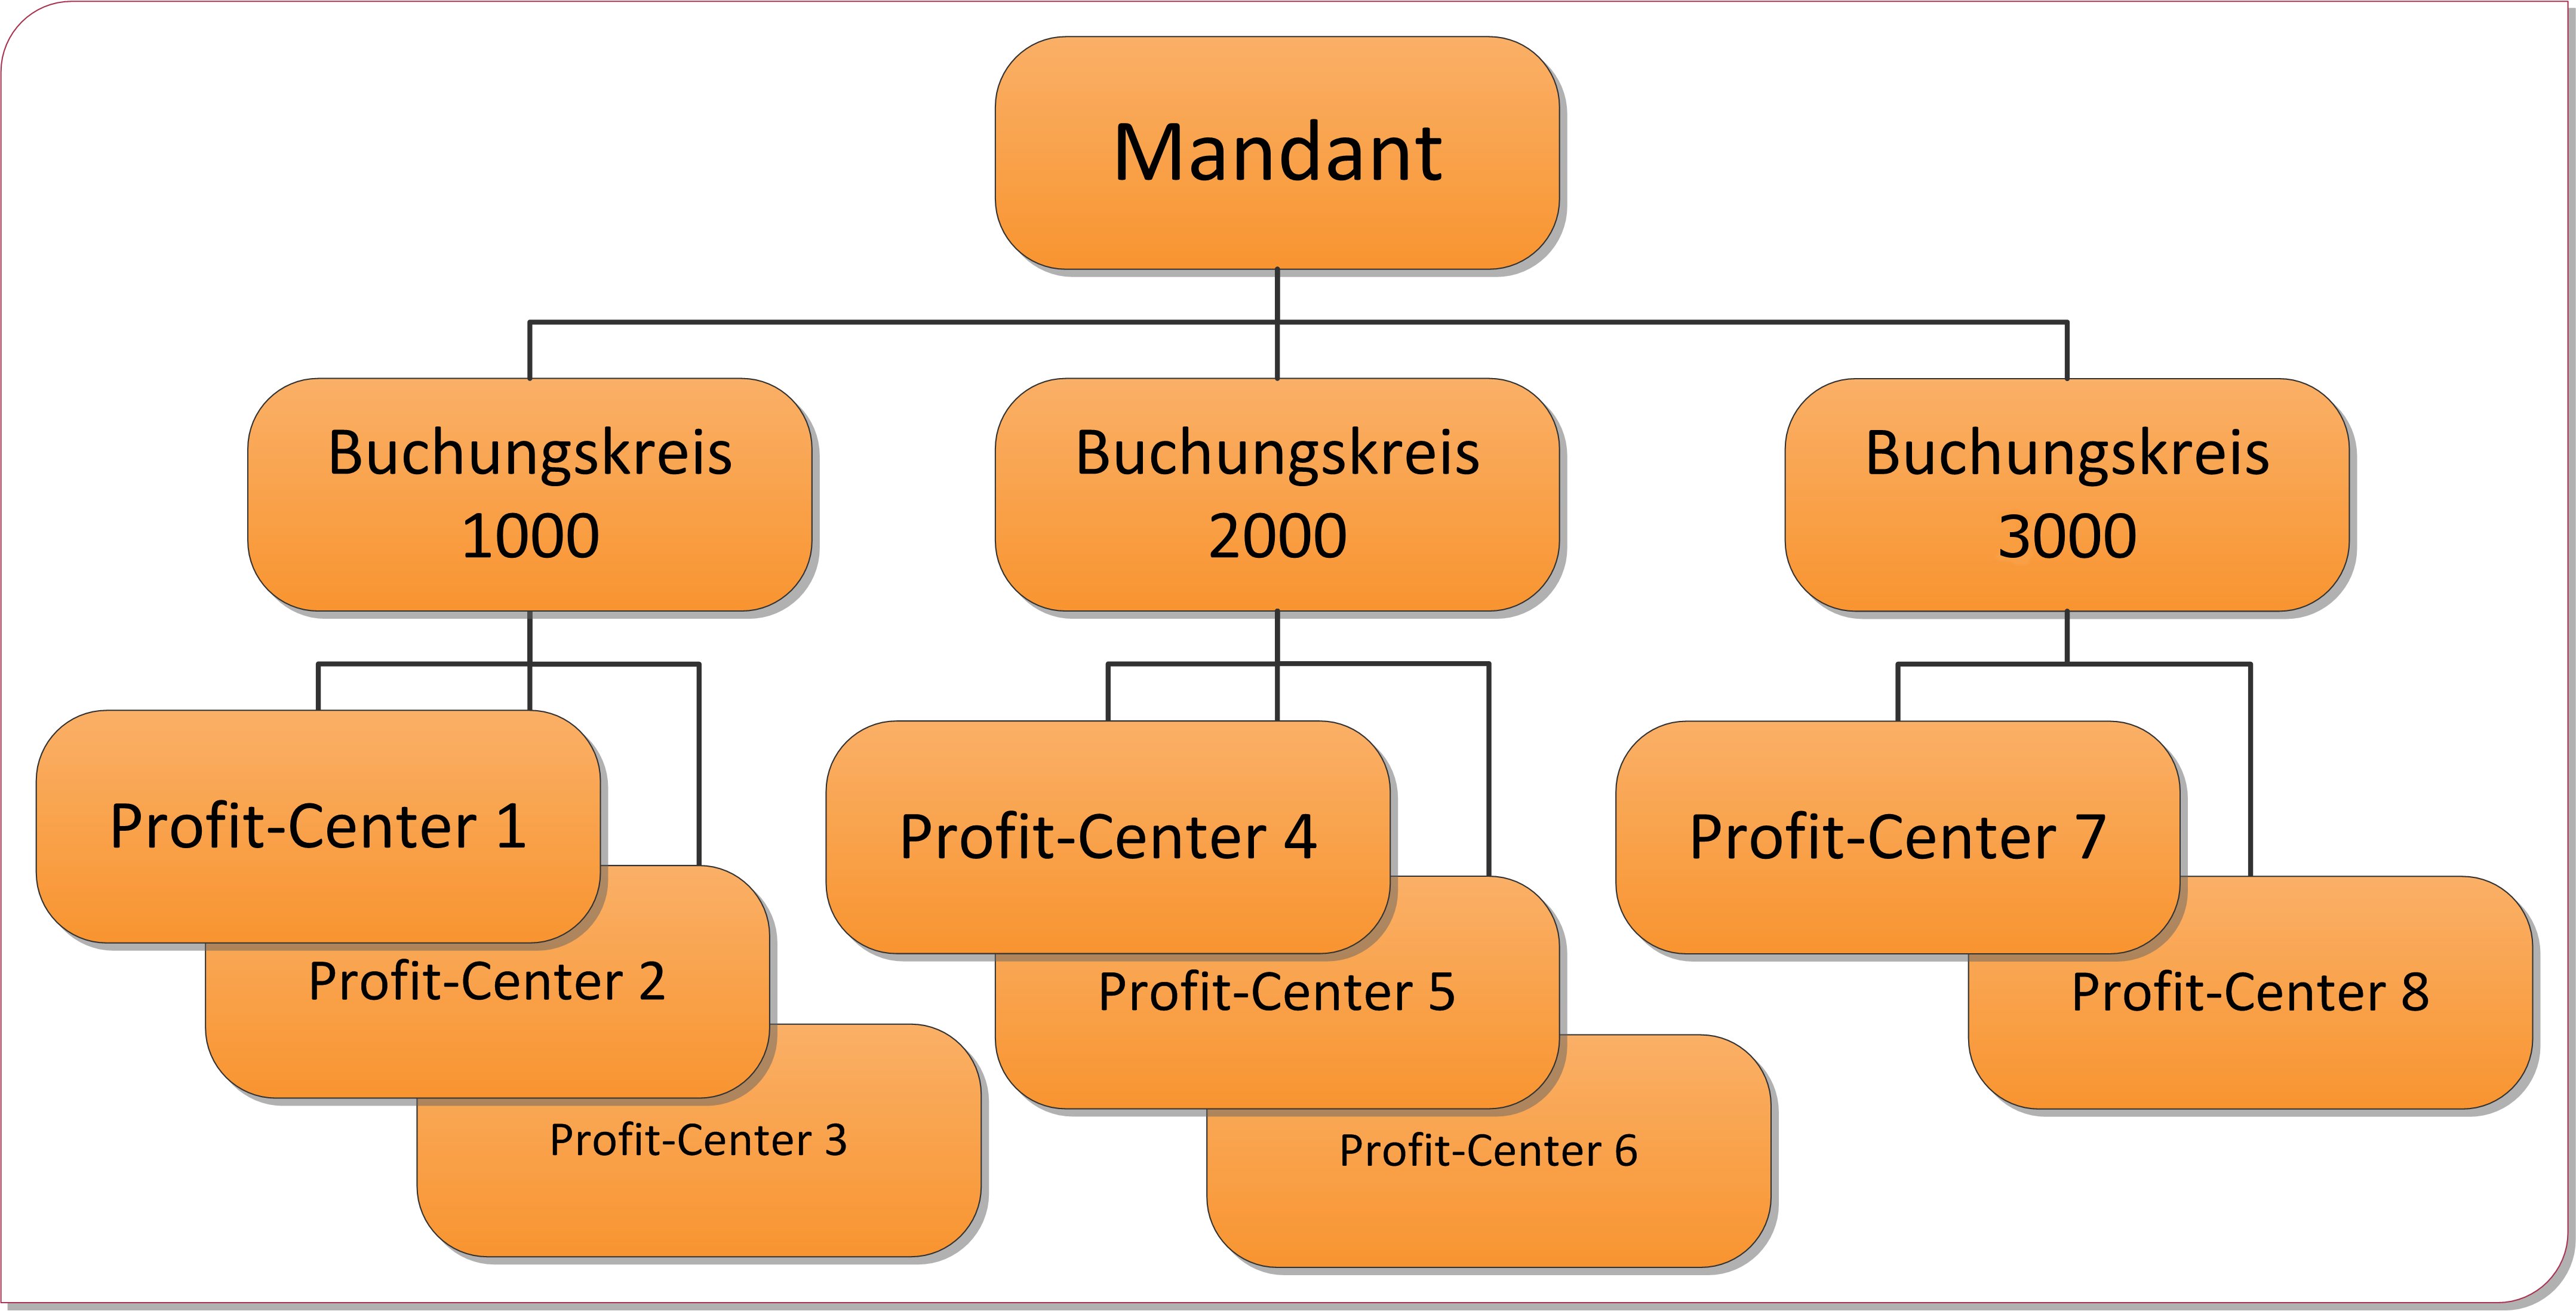
\includegraphics[width=0.9\textwidth]{Images/konzernStruktur.png}

   %{\footnotesize In Anlehnung an: \cite{Hefner2001}, S. 100}
   \caption[Konzernstruktur in SAP ERP Financials]{Konzernstruktur in SAP ERP Financials}\label{abb2}
\end{center}
\end{figure}\noindent
Die wichtigsten Organisationseinheiten innerhalb eines Mandanten sind die Buchungskreise. Unter einem Buchungskreis versteht man in SAP ERP Financials selbständig bilanzierende Einheiten der Finanzbuchhaltung. Jeder Buchungskreis erhält eine eigene Bilanz und GuV (Gewinn- und Verlustrechnung). Die Konzernabschlüsse werden ja Buchungskreis nach den geltenden gesetzlichen Anforderungen erstellt. Wenn die Unternehmung/Konzern nur aus einer Einheit zusammengesetzt sein sollte, wird in SAP ERP Financials mindestens ein Buchungskreis eingerichtet.

Der Kostenrechnungskreis dient als Organisationsstruktur vor allem dem internen Rechnungswesen und enthält mindestens einen Buchungskreis. Ein Kostenrechnungskreis wird für alle organisatorischen Einheiten vergeben, für die eine vollständige, in sich geschlossene Kostenrechnung durchgeführt werden soll. Um einen möglichst umfassenden Vergleich zu schaffen (, kommt in der Praxis meist ein einziger Kostenrechnungskreis zu Einsatz, der alle Buchungskreise des Unternehmens umfasst. Gleiches gilt auch für den Ergebnisbereich des internen Rechnungswesens.

Die Organisationsebene Geschäftsbereich wird zu Auswertungszwecken eingesetzt. Er wird nicht mehr weiter entwickelt und diente als zusätzliche Möglichkeit, Konzernabschlüsse auf Grundlage zentraler operativer Bereiche (z. B. Produktlinien, Zweigstellen oder strategische Geschäftseinheiten) zu erstellen, welche jedoch nicht den Anforderungen externer Bilanzen und GuV entsprechen. In neueren Implementierungen wird für die Segmentberichterstattung auf andere Organisationseinheiten (z. B. Profit-Center oder Segmente) zurückgegriffen.

Profit-Center sind verwaltungsorientierte Konzernstrukturen (z. B. Bereiche oder Abteilungen). Profit-Center ermöglichen, anhand der Gegenüberstellung gebuchter Kosten und Erlöse, eigene interne Betriebsergebnisse und Abschlüsse.

Für einzelne Segmente, die durch klassifizierende Merkmale beschrieben werden (z. B. Artikelgruppe, Kundengruppe, Land, Vertriebsweg), kann ein Ergebnis ausgewiesen werden. Die Segmente werden deshalb Ergebnisobjekte genannt. Obwohl bei der Definition von Segmenten keine Einschränkungen gelten, werden sie in der Regel von Profit-Centern abgeleitet und dienen in allen Gesellschaften zu Berichtszwecken. 

Um die Betriebsaufwendungen der GuV im Umsatzkostenverfahren entsprechend betrieblicher Funktionen wie Finanzen, Personalwirtschaft, Beschaffung und Logistik, Produktion oder Vertrieb gruppiert auszuweisen, kann die Organisationseinheit Funktionsbereich verwendet werden\footnote{Vgl. \cite{Hefner2001}, S. 99 ff.}\footnote{Vgl. \cite{Friedl2008}, S. 29 ff.}\footnote{Vgl. \cite{Maassen2006}, S. 71 ff.}\footnote{Vgl. \cite{Patel2009}, S. 37 ff.}\footnote{Vgl. \cite{Padhi2011}, S. 16}\footnote{Vgl. \cite{SAPFI2001}, S. 18}\footnote{Vgl. \cite{Jandt2008}, S. 101 f.}.

\subsection{Financial Accounting (FI)} %FI
Das Modul Financial Accounting (FI) lässt sich in der SAP ERP Solution Map unter SAP ERP Financials einordnen (s. Kapitel \ref{sec:Komponenten}). 
Hier werden die, in Kapitel \ref{ssec:externesRechnungswesen} externes Rechnungswesen auf Seite \pageref{ssec:externesRechnungswesen}, beschriebenen Funktionen in SAP ERP Financials abgebildet\footnote{Vgl. \cite{SAPBusinessMaps2010}}. Das Modul beinhaltet, im sogenannten General Ledger (Hauptbuch s. Kapitel \ref{sec:gl}), die Sachkontenbuchhaltung mit umfassenden Leistungen und Fähigkeiten. In der Nebenbuchhaltung werden die Accounts receivable and payable (Debitoren- und Kreditorenbuchhaltung), sowie das Asset Accounting (Kapitalanlagenbuchhaltung) geführt. 
%In SAP ERP Financials findet sich ebenfalls das Management Accounting (Kapitel 3.4) wieder. Anhand dieser beiden Module von SAP ERP Financials wird das interne und externe Rechnungswesen (Finanzbuchhaltung) einer Unternehmung abgebildet. 
%Das Interne Rechnungswesen wird unter Management Accounting (Modul CO) und das externe Rechnungswesen wird unter Financial Accounting (FI) geführt. 
Alle Buchhaltungsbestandteile finden sich im SAP ERP Financials im übergeordneten Modul Financial Accounting wieder\footnote{Vgl. \cite{SAPBusinessMaps2010}}. 

Die gesamten im Unternehmen vorkommende Informationen und Daten bzw. Buchungen lassen sich in die Hauptbereiche Materialwirtschaft, Produktion, Anlagenwirtschaft, Vertrieb und Personalwirtschaft unterteilen. Diese Datenströme aus geschäftlichen Aktivitäten können im Controlling weiter genutzt und im Sinne einer Unternehmens interne Auswertung weiter analysiert werden.

\subsubsection{General Ledger} \label{sec:gl}%Hauptbuch FI-GL -- #### ERST GEGEN ENDE SCHREIBEN!! Das neue Hauptbuch in FI vereint Funktionen aus FI und CO

Das Hauptbuch (FI-GL) bietet dem Anwender ein Gesamtbild auf die verschiedenen Konten im Rahmen des externen Rechnungswesen\footnote{Vgl. \cite{SAPGL2001}, S. 12 ff}. Das Hauptbuch bedient die Anforderungen des Gesetzgebers nach IFRS-Standard und den GoB (Grundsätzen ordnungsgemäßer Buchführung)\footnote{Vgl. \cite{SAPGL2001}, S. 14}\footnote{Vgl. \cite{SAPGL2001}, S. 23}. Im wesentlichen weißt das Hauptbuch die Unternehmensbilanz aus und stellt die GuV dar\footnote{Vgl. \cite{SAPGL2001}, S. 13}. Ebenso wird die Sachkontenbuchhaltung geführt. Alle Geschäftsfälle werden im Hauptbuch summierend mit gebucht\footnote{Vgl. \cite{SAPGL2001}, S. 12 ff}\footnote{Vgl. \cite{FICOForum2012}}\footnote{Vgl. \cite{SAPGL2001}, S. 56}. 

In der Subledger (Nebenbuchhaltung) werden hingegen Einzelposten (Positionen) erfasst. Bestandteile des Subledger sind Asset Accounting, sowie die Debitorenbuchhaltung und Kreditorenbuchhaltung. Positionen der Nebenbuchhaltung finden sich im Hauptbuch als Mitbuchung wieder und gehen jeweils auf Konten wie Forderung oder Verbindlichkeiten-Konten im Hauptbuch ein.

Im General Ledger werden Sachkontenstammdaten als sogenannte zeitüberdauernden Daten eines Sachkontos festgelegt\footnote{Vgl. \cite{SAPGL2001}, S. 25}. Der Kontenplan und das Kontenplanverzeichnis werden als Verzeichnis der "[…]Sachkontenstammsätze, die in einem Buchungskreis oder in mehreren Buchungskreisen benötigt werden" geführt\footnote{Vgl. \cite{SAPGL2001}, S. }. "Der Kontenplan enthält zu jedem Sachkontenstammsatz die Kontonummer, die Kontobezeichnung und steuernde Informationen"\footnote{Vgl. \cite{SAPFIGL}, S. 25}\footnote{Vgl. \cite{Schuler2006}, S. 51}. Hierbei kann ein operativer, zentraler oder dezentraler Kontenplan erstellt werden\footnote{Vgl. \cite{SAPGL2001}, S. 33 ff}. Mittels Einsatz von Kontengruppen können Konsolidierungen von Eigenschaften bezüglich der Verwaltung von Stammdaten, Debitoren/- und Kreditorenbuchhaltung oder Sachkonten vorgenommen werden.


\subsubsection{Accounts receivable and payable} %Debitoren FI-AR %Kreditoren FI-AP
Die Debitoren- und Kreditorenbuchhaltung findet sich in SAP unter dem Modulen FI-AP/AR wieder.
Die Debitorenbuchhaltung befasst sich im Rahmen der Finanzbuchhaltung mit der Bearbeitung von offenen Forderungen aus Lieferungen und Leistungen. Debitoren sind Kunden eines Unternehmens die offenen Rechnungspositionen beim Unternehmen noch begleichen müssen. Die Debitoren besitzen dennoch den Status eines Kunden und nicht eines Schuldners. Geschäftsbeziehungen finden weiterhin statt, werden aber in einem gesonderten Konto geführt (Risikobetrachtung z.B. Insolvenz). Das Zahlungsverhalten von Debitoren wird beobachtet und hängt mit dem betrieblichen Mahnwesen zusammen. SAP bietet zu Überwachung Alarmreport und Fälligkeitsraster an. Außerdem können Lastschriftverfahren und Anzahlungen sowie Mahnung und Schriftverkehr automatisiert angewiesen werden. Vorgänge werden dokumentiert und stehen als Saldenlisten, Journale, Kontenschreibung und andere Auswertungen zur Verfügung. Debitorenstammdaten können zentral angelegt werden und dienen zur Erfassung der für die Geschäftsbeziehung nötigen Daten des Debitors. Die Stammdatensätzen liegen zentral vor und können so übergreifend in anderen Integrationen verwendet werden wie z.B. bei Vertriebscontrolling (SD). Die Buchung eines Geschäftsfall im Rahmen der Debitorenbuchhaltung erzeugt üblicherweise einen Beleg, ebenso finden sich diese in der Hauptbuchhaltung (General Ledger) unter Berücksichtigung des geeigneten Sachkonto wieder, somit werden alle kundenbezogengen Aktivitäten (Stornierungen, Kundenzahlungen) in der Module der Debitorenbuchhaltung behandelt. 

Die Kreditorenbuchhaltung behandelt im Allgemeinen die Belange der Kreditoren, also die der Gläubiger wie z.B. Lieferanten. Die Gläubiger tragen das sogenannte Kreditorenrisiko von Forderungen aus Lieferungen und Leistungen hinsichtlich Zahlungseingangs von Waren. Dieses Kreditorenrisiko kann mittels der Kreditorenbuchhaltung überwacht und verwaltet werden. Das Cash Management und die Liquiditätsplanung eines Unternehmens werden bedient. \glqq Aus den operativen Vorgängen werden die Buchungen automatisch angestoßen\grqq
Im Rahmen des Kreditorenmanagment werden ebenfalls die Kreditorenstammdaten geführt, welche zur Erfassung aller Kreditoren dient. Der Kreditorenstammsatz kann entweder zentral oder nur für den Buchungskreis gültig angelegt werden. Stammdatenänderungen müssen nur einmalig vorgenommen werden und sind dann übergreifend z.B. in der Buchhaltung und Einkauf gültig. Typische Informationen sind Name, Adresse, Sprache, Telefonnummer, Steuernummer, Zahlungswege -empfänger und Bedingungen sowie verschiedene Einkaufsdatensätze. 
Informationen zu Konten der Kreditoren werden geführt und verwaltet, wie z.B. abweichender Zahlungsempfänger. Ebenso bietet die Kreditorenbuchhaltung die Sperrung von Konten. Kontensaldi können gebildet, und einzeln Posten angezeigt werden. Im Rahmen einer Kontoanalyse wird das Zahlungsverhalten somit transparent gemacht. Dies ist relevant, um Risiken zu erkennen und geeignete Kredite vergeben zu können. Zu analysezwecken können auch Simulationen gefahren werden. Der Leistungsumfang der Kreditorenbuchhaltung umfasst u.a. weiterhin die Bearbeitung von Gutschriften, Storno, Anzahlungen, Bürgschaften, Vorsteuer, Fremdwährung, Mahnungen.
Wie auch in der Debitorenbuchhaltung werden die Buchungen der Kreditorenbuchhaltung werden auch in der der Hauptbuchhaltung (General Ledger) geführt und je nach Art auf das jeweilige Sachkonto geschrieben.



\subsubsection{Tax Accounting} %Steuern
\footnote{Vgl. \cite{SAPFIAPAR2006}} %für Bezug zu interat. Steuerrecht und sonst. Features

\subsubsection{Bank Accounting} %Bankbuchhaltung FI-BL
Das Modul Bankbuchhaltung (FI-BL) (engl. Bank Accounting) dient zur Abwicklung von Geschäftsfällen mit Bankenbeteiligung (Zahlungen) zwischen den Geschäftspartnern. 
Im Bankenverzeichnis werden im die Bankenstammdaten abgebildet, diese beinhalten die typischen Informationen für die für die Abwicklung eines Bankgeschäfts. Bankenverzeichnisse können maschinell importiert sowie manuell angelegt werden. Die geführten Bankenstammdaten können wie üblich editiert werden, so dass nachträgliche Anpassungen möglich sind. Dies wäre z.B. bei einer Stammdatenpflege relevant. Neben der Bankenstammdaten ist die Belegung der Bankverbindung in Verbindung mit der Debitoren und Kreditorenstammdaten nötig, um für Debitoren und Kreditioren den Zahlungsverkehr ausführen zu können. Diese Angaben können ebenfalls buchungskreisspezifisch hinterlegt werden. 
Weiterhin können mit der Bankbuchhaltung verschiedene Bankwege(z.B. mehrstufige Zahlwege) bedient werden und diese ebenso für das Cashmanagement definiert werden. Das Modul bietet eine umfassende Scheck- und Wechselverwaltung, welcher als Sonderhauptbuchvorgang detailliert werden kann. Insgesamt werden Aufgaben zum Zahlungsverkehr geführt wie z.B. die Fähigkeiten der Kassenbuchverwaltung Nutzung von Kontoauszügen.

Das Modul Bankbuchhaltung (FI-BL) dient zur Abwicklung von Geschäftsfällen mit Bankenbeteiligung (Zahlungen) zwischen den Geschäftspartnern. Im Bankenverzeichnis werden im die Bankenstammdaten abgebildet, diese beinhalten die typischen Informationen für die für die Abwicklung eines Bankgeschäfts. Bankenverzeichnisse können maschinell importiert sowie manuell angelegt werden. Die geführten Bankenstammdaten können wie üblich editiert werden, so dass nachträgliche Anpassungen möglich sind. Dies wäre z.B. bei einer Stammdatenpflege relevant. Neben der Bankenstammdaten ist die Belegung der Bankverbindung in Verbindung mit der Debitoren und Kreditorenstammdaten nötig, um für Debitoren und Kreditioren den Zahlungsverkehr ausführen zu können. Diese Angaben können ebenfalls buchungskreisspezifisch hinterlegt werden. Weiterhin können mit der Bankbuchhaltung verschiedene Bankwege(z.B. mehrstufige Zahlwege) bedient werden und diese ebenso für das Cashmanagement definiert werden. Das Modul bietet eine umfassende Scheck- und Wechselverwaltung, welcher als Sonderhauptbuchvorgang detailliert werden kann. Insgesamt werden Aufgaben zum Zahlungsverkehr geführt wie z.B. die Fähigkeiten der Kassenbuchverwaltung Nutzung von Kontoauszügen.

\subsubsection{Asset Accounting} %Anlagenbuchhaltung FI-AA
Das Asset Accounting dient im Allgemeinen dazu, dass Vermögen im Anlagevermögen in der Bilanz (gem. HGB) der Unternehmung zu verwaltet. Anlagevermögen sind langfristige Wertanlagen die Kapital binden wie z.B. Gebäude, Fuhrpark etc. Die Anlagenbuchhaltung kann individuell an die speziellen Anforderungen angepasst (Customizing) werden. 
Die Anlagenbuchhaltung steht in komplexen Wechselbeziehungen mit anderen Modulen und kann mit Komponenten wie Material Management, Finanzbuchhaltung, Profit Centern und Fertigung verbunden werden. Die Anlagenbuchhaltung kann verschiedene Organisationseinheiten wie Gliederung mittels länderspezifischen Bewertungsplan und Kontenplan-Struktur abbilden, sowie Buchungskreisen zugeordnet werden.
Neben dieser Fähigkeit der Integration zählt zu den Hauptaufgaben die Gliederung des Anlagevermögens nach anlagenbezogenen, klassifizierenden und bilanziellen Strukturen, anhand deren sich je nach Anforderung Aussagen bezüglich der Werteermittlung treffen lassen. Die Bewertungsbereiche dienen dazu das Anlagevermögen für unterschiedliche Interessen wie bilanziellen, kalkulatorischen oder steuerlichen Anfordeurngen bewerten zu können.
Im Rahmen des Asset Accounting werden ausserdem die Geschäftsjahre und Perioden berücksichtigt, um mit der Periodensteuerung u.a. die Abschreibungszeiträume abbilden zu können. Neben der Berücksichtigung der verschiedenen Abschreibungsarten und der Zinsrechnung und Vermögensteuer, bietet das Modul FI-AA den Asset Explorer, um aktuelle Werte der Anlagen darstellen zu können. Grundsätzlich werden im Asset Accounting der Abgang von Anlagen sowie, Anlagenumbuchungen und Anlagentransfers aber auch die Erstellung von Inventurlisten zu Verfügung gestellt. 
Hinsichtlich Jahresabschluss des Unternehmens ist die Anlagenbuchhaltung maßgeblich beteiligt. Bei Abschluss des Buchungskreises können in der Anlagenbuchhaltung keine Buchungen mehr erfolgen.


\subsection{Management Accounting (CO)} %CO
Das Modul Management Accounting (Controlling -- CO) bildet die, in Kapitel \ref{ssec:internesRechnungswesen} internes Rechnungswesen auf Seite \pageref{ssec:internesRechnungswesen}, beschriebenen Funktionen in SAP ERP Financials ab und gliedert sich in die drei Komponenten Overhead Cost Controlling (CO-OM), Product Cost Accounting (CO-PC) und Profitability Analysis (CO-PA). Abbildung \ref{abb3} auf Seite \pageref{abb3} zeigt die vollständig in der Finanzbuchhaltung und Kostenrechnung integrierten Komponenten. 
\begin{figure}[htbp]
\begin{center}
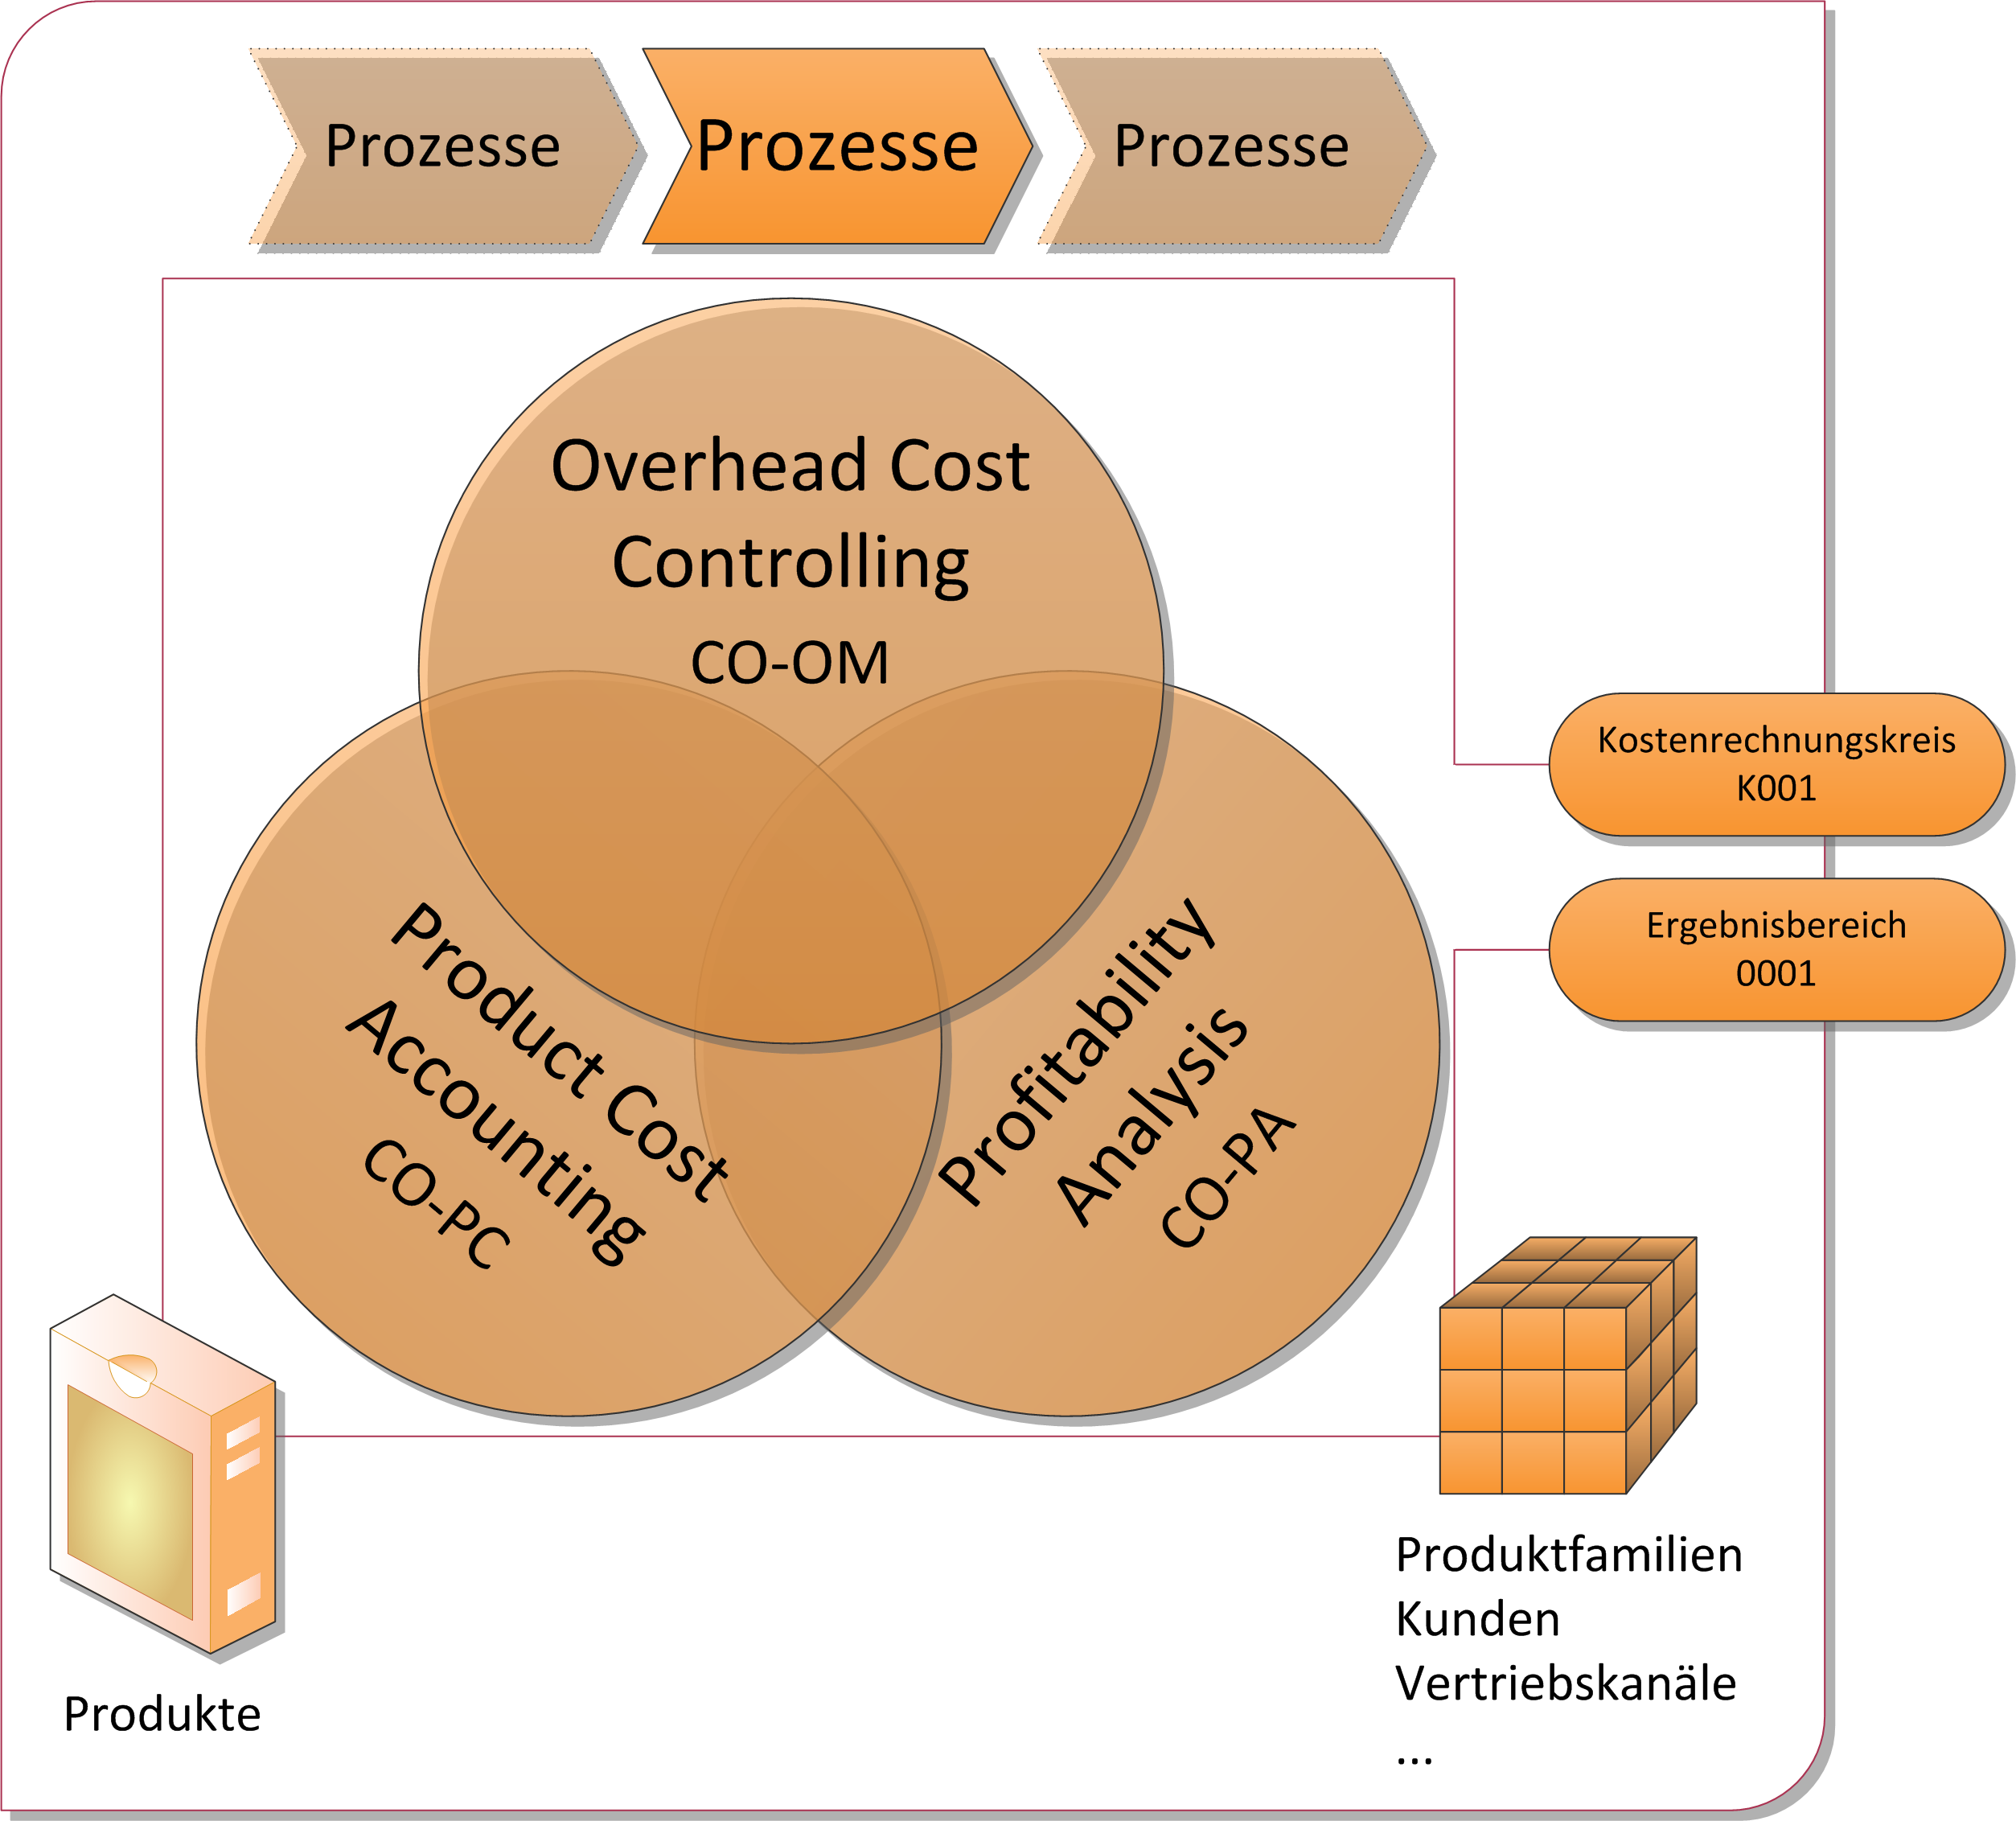
\includegraphics[width=0.8\textwidth]{Images/managementAccounting.png}

   {\footnotesize In Anlehnung an: \cite{SAPCOOMABC2001}, S. 11}
   \caption[Management Accounting -- Das Modul CO]{Management Accounting -- Das Modul CO}\label{abb3}
\end{center}
\end{figure}\noindent
Die zentrale Organisations- und Kontierungseinheit im Controlling ist der Kostenrechnungskreis (Vgl. s. Abb. \ref{abb4}, S. \pageref{abb4}). Mithilfe des Kostenrechnungskreises können Sie Ihr Unternehmen im Hinblick auf die Kostenrechnung im SAP-System buchungskreisübergreifend struktuieren\footnote{Vgl. \cite{Patel2009}, S. 291}\footnote{Vgl. \cite{Friedl2008}, S. 23}\footnote{Vgl. \cite{Klein2010}, S. 99}. SAP ERP stellt verschiedenen Kostenträger zur Verfügung, um alle anfallenden Kosten und Erlöse im Unternehmen zu strukturieren und möglichst exakt darstellen zu können. Der Begriff Kostenträger bzw. Kostensammler beschreibt Objekte wie Kostenstellen, Kostenarten und Innenaufträge\footnote{Vgl. \cite{Patel2009}, S. 208}. 
\subsubsection{Overhead Cost Controlling}
\abk{Cost Center Accounting}{dt. Kostenstellenrechnung (Unterkomponente CO--OM--CCA)}
\abk{Internal Order Accounting}{dt. Innenaufträge (Unterkomponente CO-OM-OPA)}
\abk{Profit Center Accounting}{Profit-Center Rechnung (Komponente EC-PCA}
\abk{Overhead Cost Controlling}{dt. Gemeinkostenrechnung (Komponente CO-OM)}
\begin{floatingfigure}[htbpr]{0.5\textwidth} 
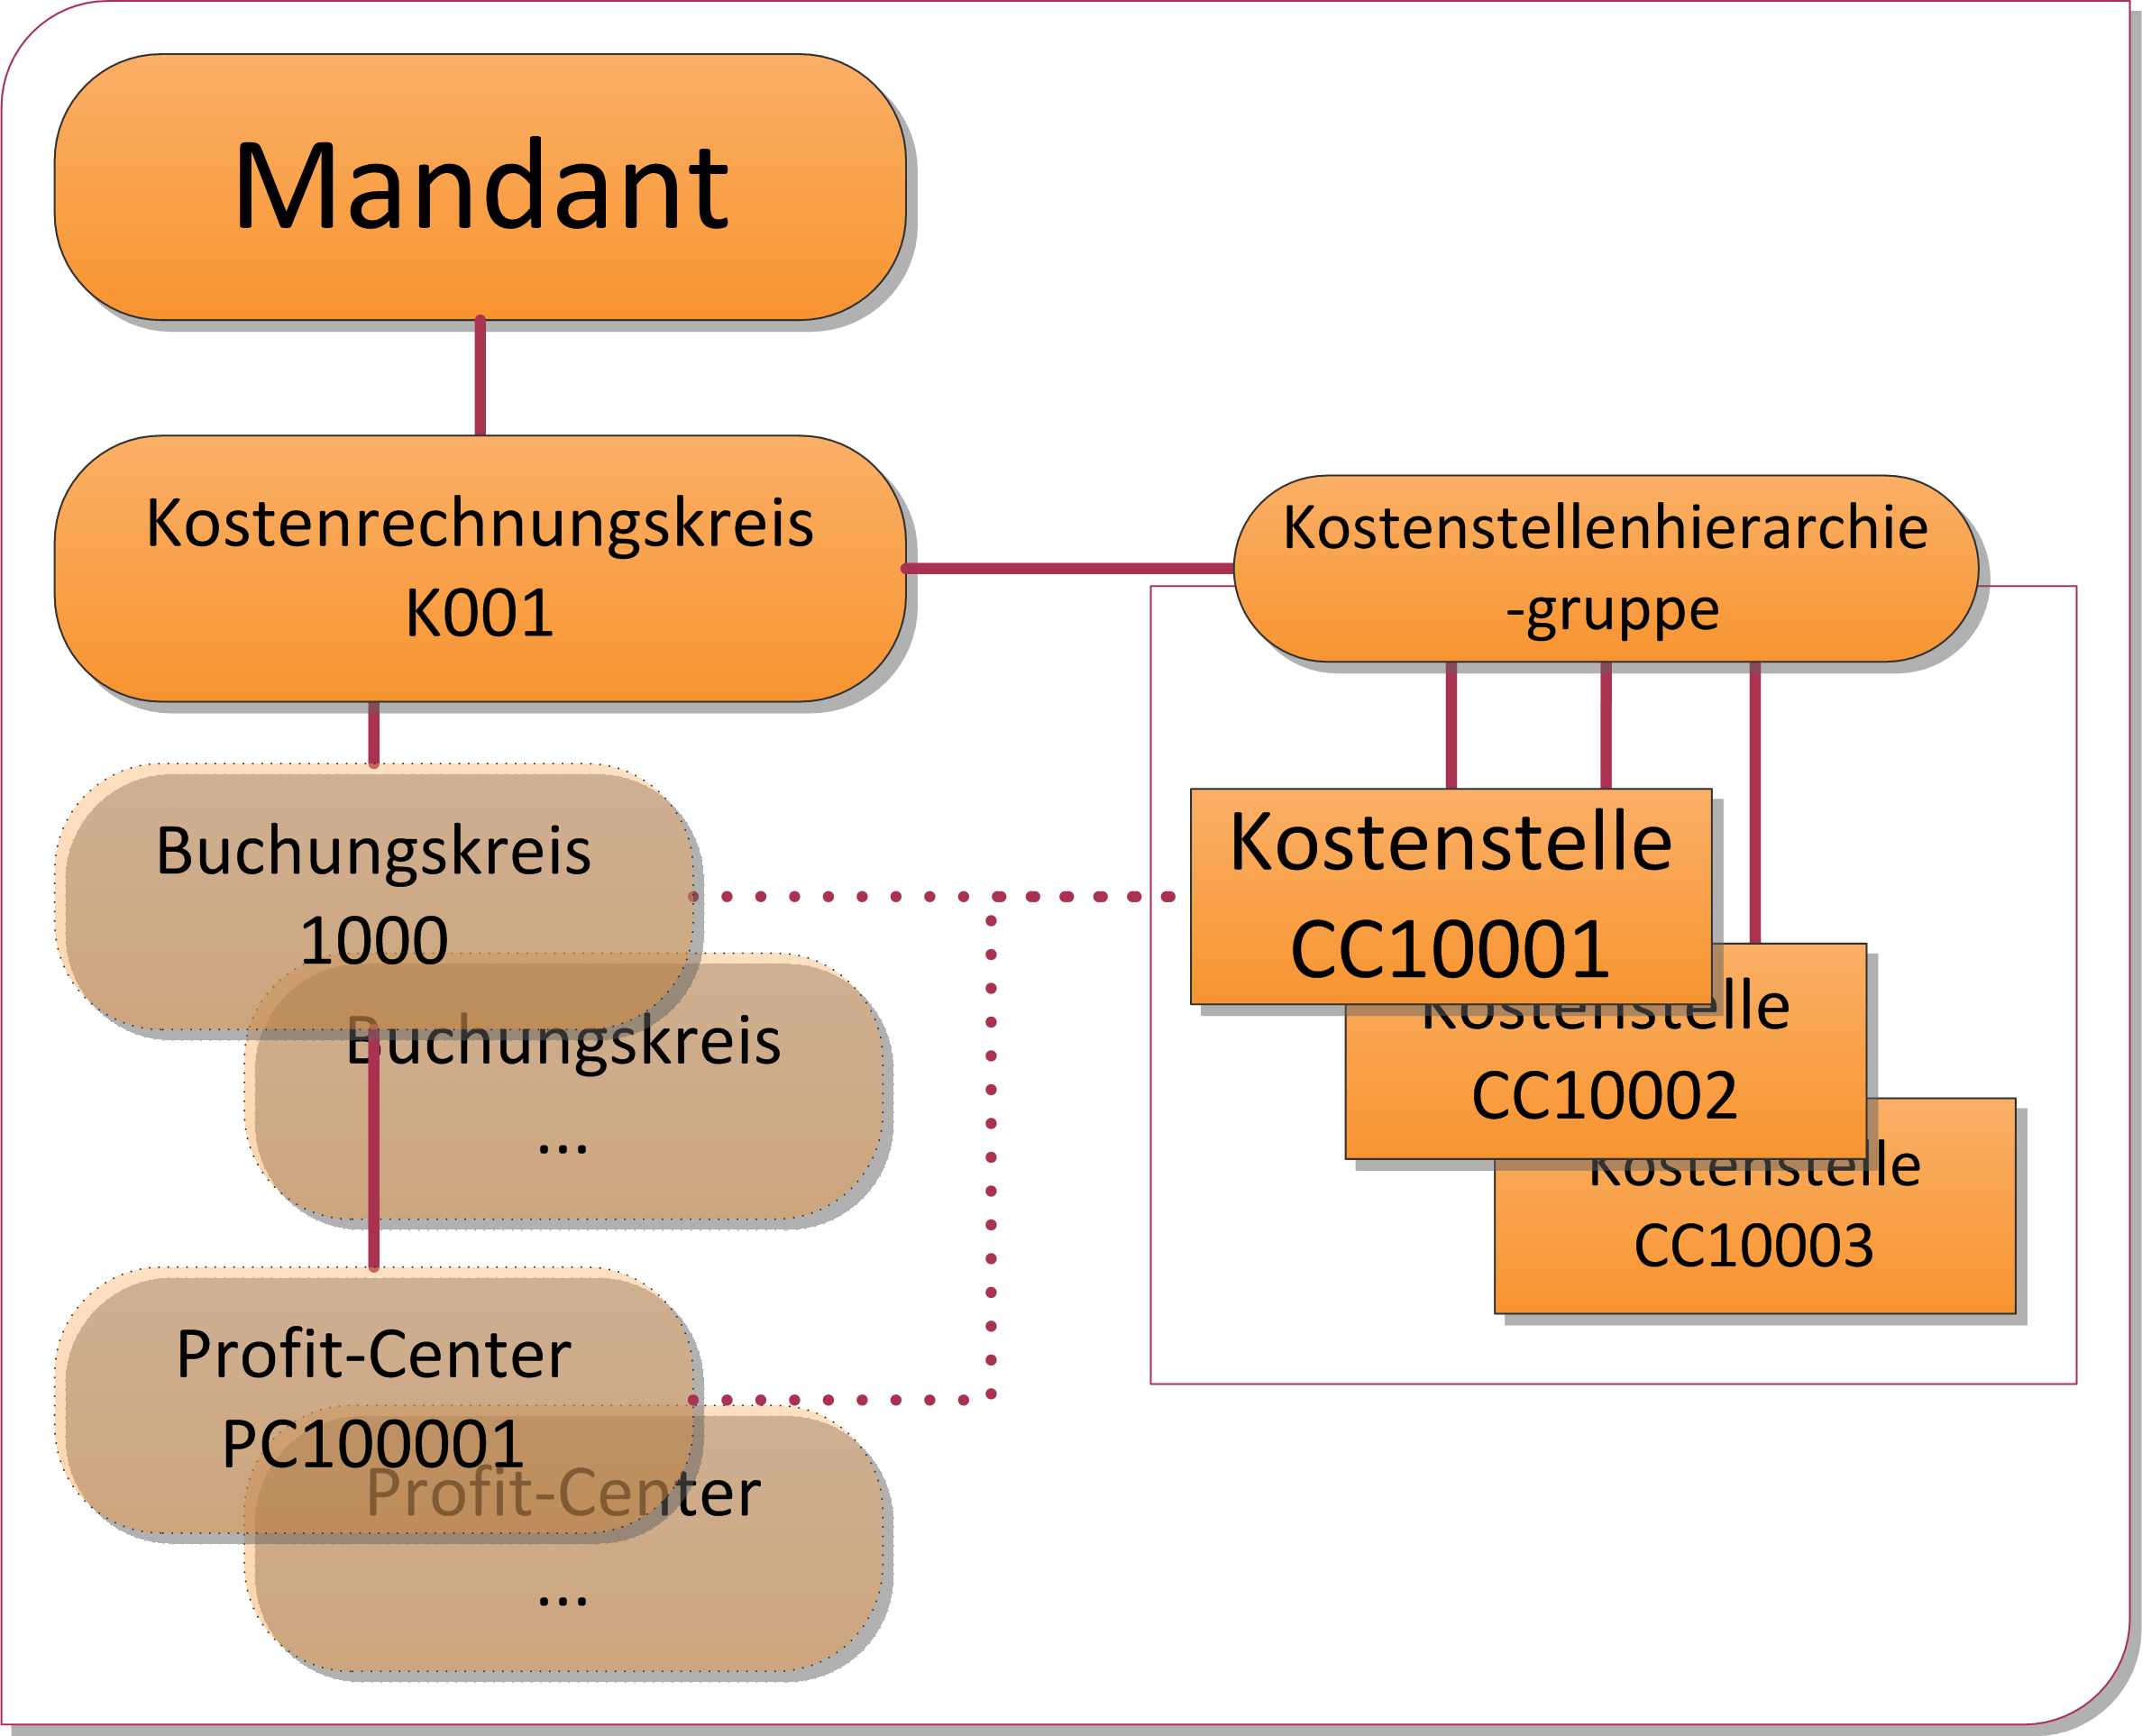
\includegraphics[width=0.5\textwidth]{Images/kostenRechnungskreis.png}
\begin{flushright}
   %{\footnotesize In Anlehnung an: \cite{Hefner2001}, S. 100}
   \caption[Kostenrechnungskreis in SAP ERP Financials]{Kostenrechnungskreis in \\SAP ERP Financials}\label{abb4}
\end{flushright}
\end{floatingfigure}\noindent
Overhead Cost Controlling (dt. Gemeinkostenrechnung) ist vor allem den Gemeinkosten gewidmet. Als Gemeinkosten\footnote{Personalkosten, Anlagekosten, Reisekosten, Beschaffungskosten, usw. - s. a. \cite{Baier2009}, S. 554} werden in der Regel Kosten bezeichnet, die im Gegensatz zu den direkten Kosten, nicht direkt den Produkten oder Dienstleistungen zugeordnet werden können. SAP ERP Financials unterstützt überwiegend mit der Kostenstellenrechnung, Innenauftragsrechnung und Prozesskostenrechnung die genaue Aufzeichnung, Analyse, Verrechnung und Buchung von Gemeinkosten\footnote{Vgl. \cite{Patel2009}, S. 288}\footnote{Vgl. \cite{SAPCOOMCCA2001}, S. 18}. 

Als Fundament des Controllings in SAP gilt die Kostenstellenrechnung\footnote{Vgl. \cite{Klein2010}, S. 98}.
Die Kostenstellen in SAP werden unterhalb eines Kostenrechnungskreises in einer Kostenstellenhierarchie organisiert und entsprechen in der Regel der Struktur eines Unternehmens im Hinblick auf Büros, Abteilungen, Bereiche und Standorte. Der Kostenstellenverantwortliche wird in den Stammdaten der Kostenstellen hinterlegt und verantwortet sowohl die präzise Aufzeichnung und Abrechnung von Kosten in ihren Kostenstellen, sowie die Einhaltung des vorgesehenen Budgets. Die Integration, z. B. die automatische Kostenstellenfindung in anderen SAP Modulen, wird durch eine Zuordnung der Organisationseinheiten wie einem Buchungskreis oder einem Profit-Center ermöglicht\footnote{Vgl. \cite{Patel2009}, S. 296 f.}.
Mithilfe der Kostenstellenrechnung wird im SAP-System eine präzise Kostenplanung, -erfassung und -aggregation vorgenommen. Es erfolgt eine Zuordnung der Gemeinkosten nach ihren Kostenarten\footnote{Vgl. \cite{SAPOMCEL2001}, S. 6} auf die Kostenstellen und im Rahmen der innerbetrieblichen Leistungsverrechnung können Kosten der Vorkostenstellen auf die Endkostenstellen weiterverrechnet werden\footnote{Vgl. \cite{Friedl2008}, S. 24}. Außerdem wird eine Rückverfolgung der Kosten von den zugewiesenen Werten bis zu deren Ursprung ermöglicht. 
Auf diese Weise ist die Transparenz und Kontrolle der operativen Verfahren sichergestellt\footnote{Vgl. \cite{Patel2009}, S. 288}. 
Die Kostenstellenrechnung gibt an, wo im Unternehmen welche Kosten angefallen sind\footnote{Vgl. \cite{Friedl2008}, S. 24}.

Innenaufträge stellen eine weitere Möglichkeit zur Ermittlung der Istkosten einer internen Initiative, eines internen Jobs oder eines einfachen Projekts dar\footnote{Vgl. \cite{Patel2009}, S. 289}. Als klassisches Beispiel veranstaltet die Marketingabteilung einen Messeauftritt. Die anfallenden Kosten werden als Messekosten mit der Kostenstelle des Marketings verrechnet. In der Kostenstellenrechnung können nun Rückschlüsse auf die Kostenart und den Ursprung der Kosten gezogen werden. Wird für diesen Messeauftritt ein Innenauftrag erstellt, können die Kosten in Art und Ursprung diesem speziellen Vorgang zugeordnet und noch differenzierter betrachtet werden. Neben den Kosten können auch Messeerlöse auf den Innenauftrag verrechnet und ihnen gegenüber gestellt werden\footnote{Vgl. \cite{Klein2010}, S. 184 f.}. 
So bieten Innenaufträge im Vergleich zu Kostenstellen eine höhere Transparenz, da die Kostenanalyse für einzelne Jobs und nicht für die gesamte Kostenstelle durchgeführt wird. Innenaufträge können während des vollständigen Lebenszyklus eines Jobs überwacht werden, indem fortlaufend ein Vergleich der Istkosten und -erlöse mit den Plankosten und -erlösen stattfindet. Die für Innenaufträge anfallenden Kosten können an weitere Innenaufträge, Kostenstellen usw. weiterberechnet werden\footnote{Vgl. \cite{Patel2009}, S. 289}.

Die Geschäftsprozessplanung ist ein Vorgang, der in nahezu jedem Unternehmen anders gehandhabt wird. Branchenspezifische Besonderheiten, besondere organisatorische Strukturen und Verantwortlichkeiten erzwingen eine firmenindividuelle Gestaltung der Prozesse\footnote{Vgl. \cite{Friedl2008}, S. 24}. Einen Einblick in die Rentabilität dieser Geschäftsprozesse erlauben die zahlreichen Techniken und Methoden der Prozesskostenrechnung (CO-OM-ABC, Activity-Based Costing)\abk{Activity-Based Costing}{dt. Prozesskostenrechnung (Unterkomponente CO--OM--ABC)}. Die Prozesskostenrechnung ermöglicht es, die Istkosten von Geschäfts-prozessen, Produkten und Dienstleistungen transparent zu gestalten. Im Gegensatz zur verantwortungs- und funktionsorientierten Kostenstellenrechnung bildet sie eine vorgangsorientierte und funktionsübergreifende Sicht der Abläufe in Unternehmen ab. Dadurch ergänzt die Prozeßkostenrechnung die Kostenstellenrechnung\footnote{Vgl. \cite{SAPCOOMABC2001}, S. 11}. 
Um Betriebskosten \\präziser zu bestimmen, kann die Prozesskostenrechnung mit den operativen und logistischen Komponenten des SAP-Systems (z. B. Logistik) integriert werden. Parameter wie z. B. der Anzahl an Kreditorenrechnungen, Bestellungen oder abgewickelte Kundenbesuche werden dann zur Berechnung hinzu gezogen\footnote{Vgl. \cite{Patel2009}, S. 289}. 
Die Istkosten für Geschäftsprozesse, Produkte und Dienstleistungen werden transparent darstellt und verbessert die Produktkalkulation\footnote{Vgl. \cite{Patel2009}, S. 318 f.}.


\subsubsection{Product Cost Accounting}
\abk{Product Cost Accounting}{dt. Produktkosten-Controlling (Komponente CO-PC}
Unabhängig von der Branche bietet jedes Unternehmen ein Produkt oder eine Dienstleistung an. Die Kontrolle über die Produktkosten ist für jedes Unternehmung ein wesentlicher Aspekt der Wirtschaftlichkeit. Produkt- und Dienstleistungskosten können direkt den Produkten und Dienstleistungen zugeordnet werden. Die Komponente Produktkostencontrolling (CO-PC) orientiert sich an den Produkten der Unternehmung und dient der Erfassung der direkten Kosten, sowie deren präzisen, detaillierten und flexiblen Kalkulation. Die Kalkulationen dienen z. B. zur Senkung der direkten oder indirekten Fertigungskosten, zur Kostenschätzung für eine potenzielle neue Produktlinie oder Änderungen an vorhandenen Produkten\footnote{Vgl. \cite{Patel2009}, S. 355}.
Die SAP Komponente CO-PC gliedert sich im Wesentlichen in die Unterkomponenten Produktkostenplanung (CO--PC--PCP), Istkalkulation/Material-Ledger (Unterkomponente CO--PC--ACT), die Kostenträgerrechnung (CO--PC--OBJ) und das Informationssystem (CO--PC--IS)\footnote{Vgl. \cite{Friedl2008}, S. 25}.
\abk{Product Cost Accounting Information System}{dt. Informationssystem (Unterkomponente CO--PC--IS)}
\abk{Cost Object Controlling}{dt. Kostenträgerrechnung (Unterkomponente CO--PC--OBJ)}
\abk{Product Cost Planning}{dt. Produktkostenplanung (Unterkomponente CO--PC--PCP)}
\abk{Actual Costing/Material Ledger}{Istkalkulation/Material-Ledger (Unterkomponente CO--PC--ACT)}
Das Produktkosten-Controlling liefert Basisinformationen für folgende betriebswirtschaftliche Funktionen\footnote{Vgl. \cite{Maassen2006}, S. 346}\footnote{Vgl. \cite{Klein2010}, S. 209}\footnote{Vgl. \cite{SAPCOPCPCP2001}, S. 20}:
\begin{compactitem}
\item  Ermittlung Material-, Fertigungs- und Gemeinkosten,
\item  Ermittlung des Verkaufspreises,
\item  Bewertung des Lagerbestandes und Materialbewegungen (CO-PC-ACT), 
\item  Ermittlung der Deckungsbeiträge,
\item Profit Center-Rechnung,
\item Make or Buy - Entscheidungen,
\item Kostenvergleich zwischen einzelnen Fertigungsstandorten.
\end{compactitem}
\begin{figure}[htbp]
\begin{center}
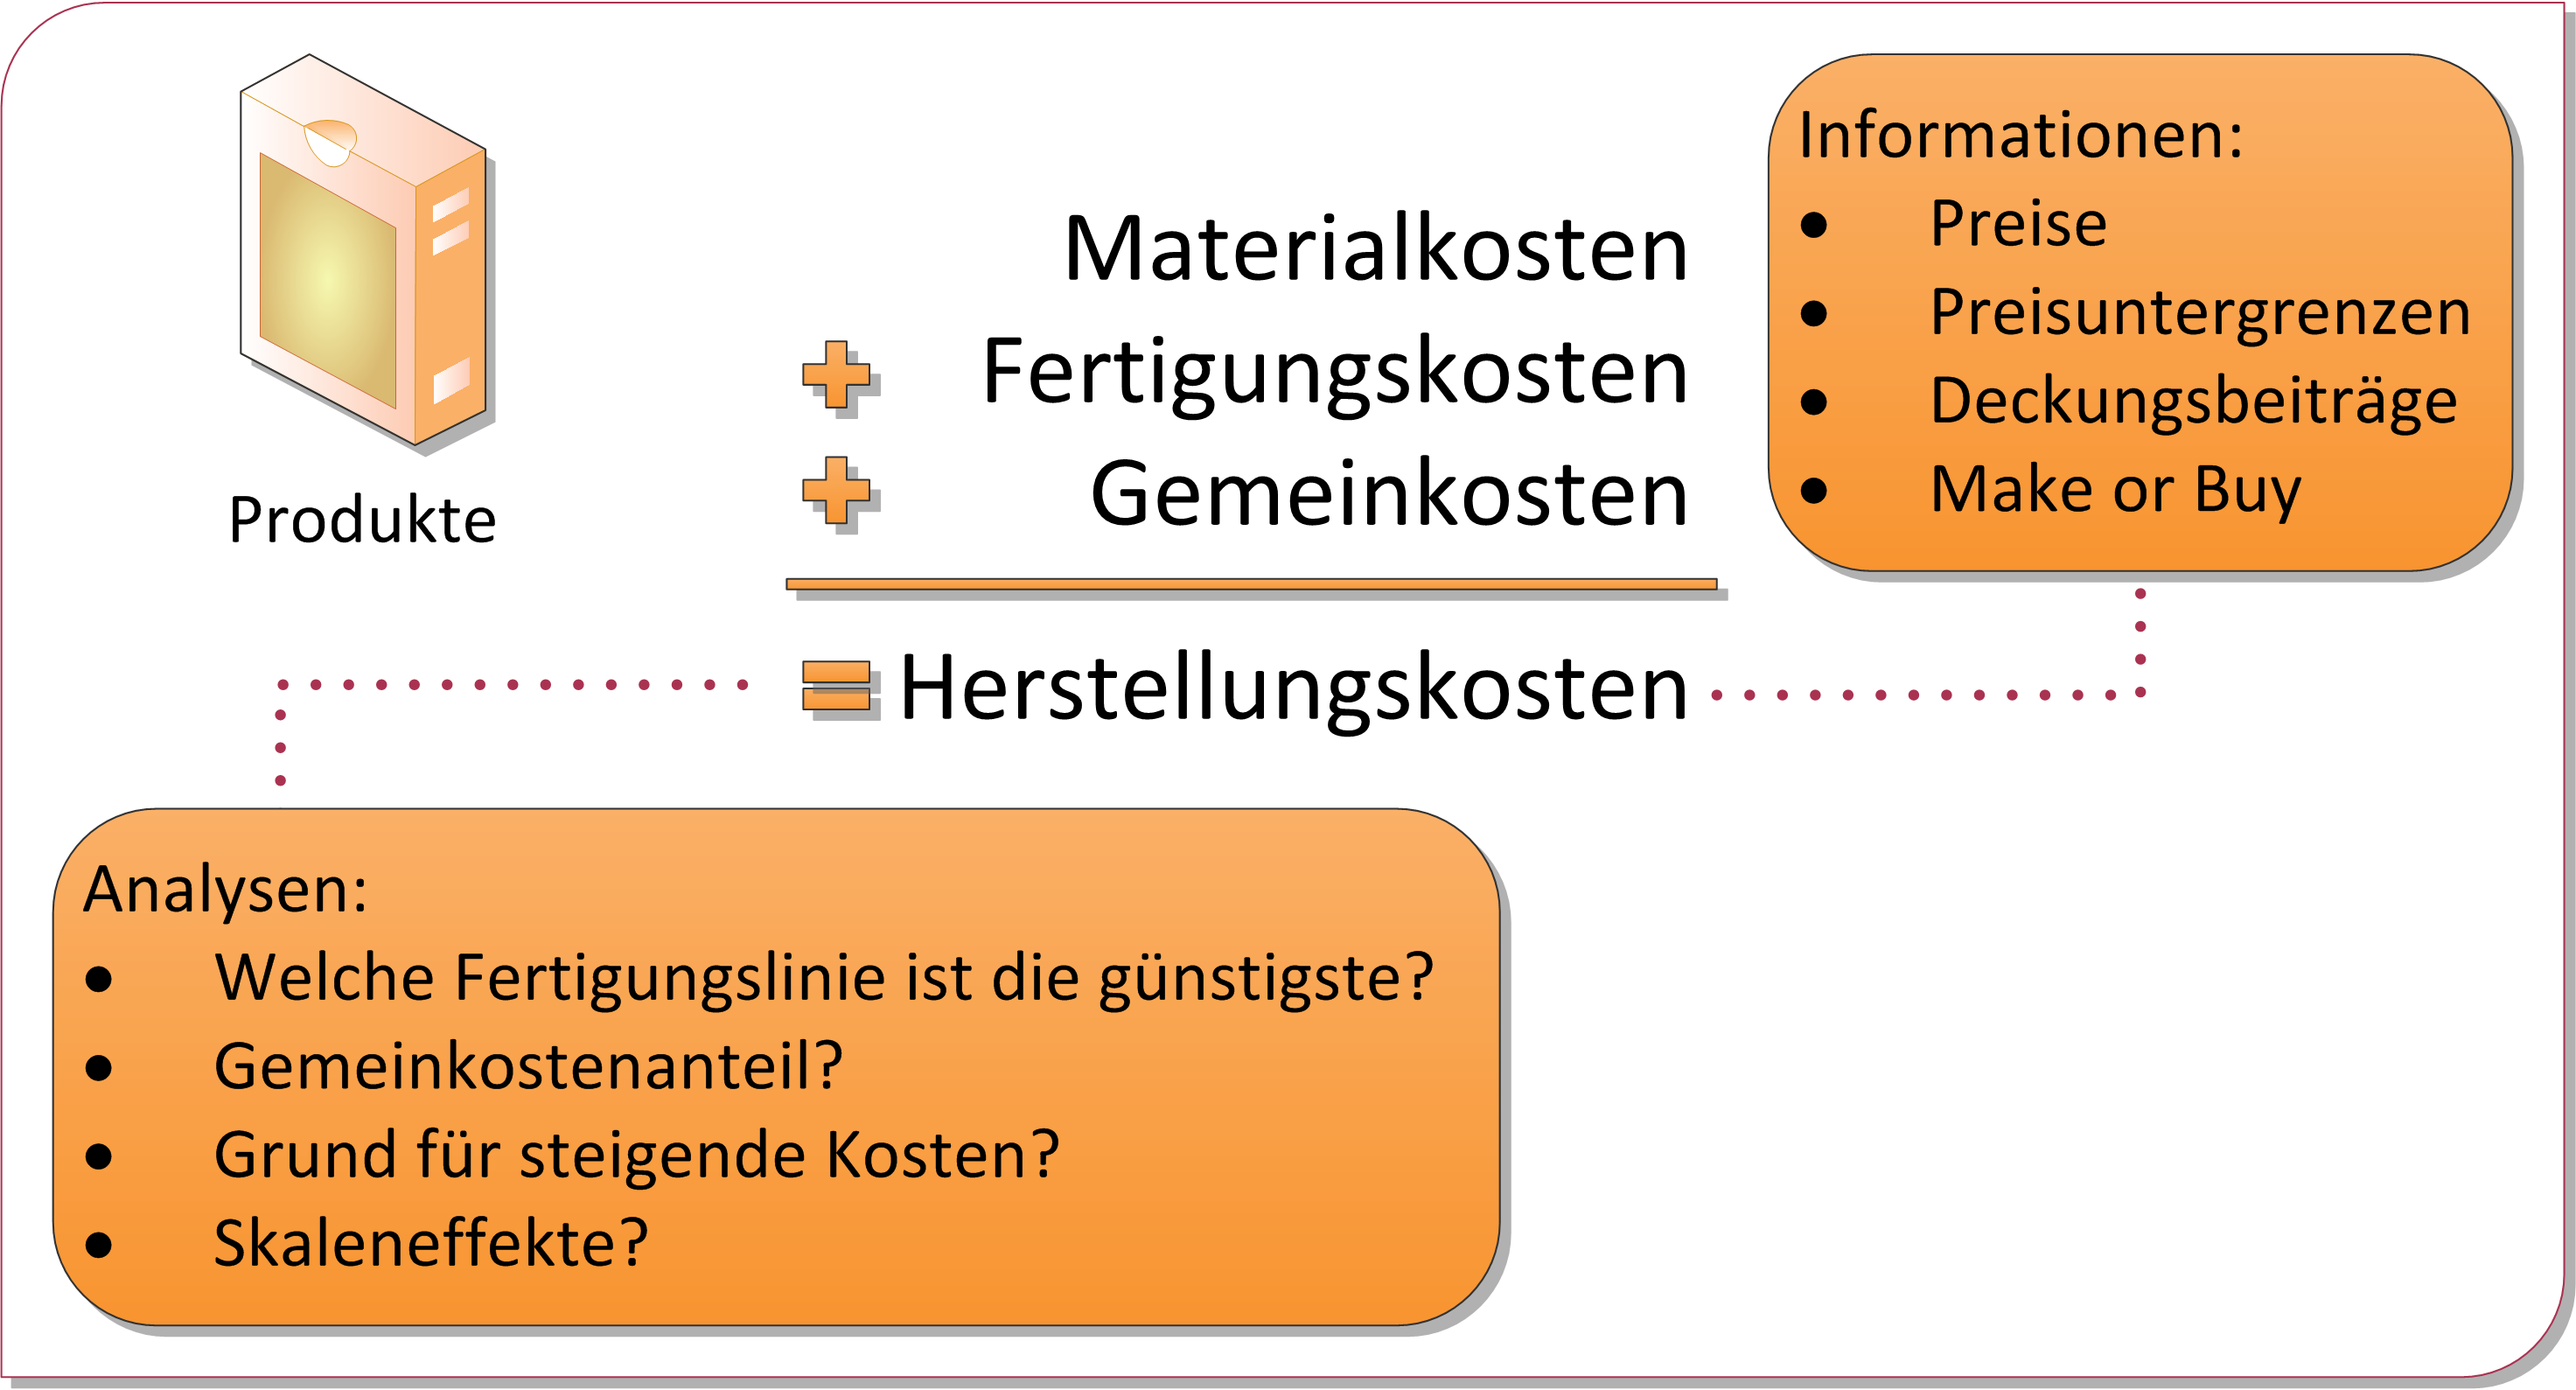
\includegraphics[width=0.8\textwidth]{Images/produktkosten.png}

   {\footnotesize In Anlehnung an: \cite{SAPCOPCPCP2001}, S. 20}
   \caption[Product Cost Accounting]{Product Cost Accounting}\label{abb3}
\end{center}
\end{figure}\noindent
In der Produktkostenplanung wird die auftragsneutrale Kalkulation der Herstellungskosten vorgenommen. Es können verschiedene Musterproduktkalkulationen durchgeführt werden. Auch kann auf Daten der SAP Produktionskomponenten (PP) zugegriffen und Arbeitspläne sowie Stücklisten in den Analysen verwertet werden\footnote{Vgl. \cite{Friedl2008}, S. 26}.

Die Kostenträgerrechnung rechnet die im Unternehmen angefallenen Kosten den Leistungseinheiten des Betriebes (z. B. Erzeugnisse, Erzeugnisgruppen, Aufträge) zu. Im Gegensatz zur Produktkostenplanung, werden in der Kostenträgerrechnung konkrete Istläufe ausgewertet und auch für die o. g. betrieblichen Planungs- und Entscheidungsprobleme eingesetzt werden\footnote{Vgl. \cite{Friedl2008}, S. 27}.

Das Informationssystem bietet zahlreiche detaillierte Berichte, die unter anderem für das Produktkostencontrolling, für das Material-Ledger und für Mischkalkulationen erstellt wurden\footnote{Vgl. \cite{Patel2009}, S. 392 f.}



\subsubsection{Profitability Analysis} %CO-PA
\abk{Profitability Analysis}{dt. Ergebnis- und Marktsegmentrechnung (SAP CO-PA)}
Die Ergebnis- und Marktsegmentrechnung (CO-PA) dient der Beurteilung von Marktsegmenten\footnote{Vgl. \cite{SAPCOPA2001}, S. 9}.
Aus ihr geht hervor, wie sich einzelne Produkte und Dienstleistungen in den unterschiedlichen Marktsegmenten behaupten und liefert Informationen zu Kunden und Produkten für den Vertrieb\footnote{Vgl. \cite{Patel2009}, S. 428}.
Ziel des Systems ist es, aus der Sicht des Markts die Bereiche Vertrieb, Marketing, Produkt-Management und Unternehmensplanung mit Informationen für das Controlling und die Entscheidungsfindung zu unterstützen\footnote{Vgl. \cite{SAPCOPA2001}, S. 9}.
Für verschiedene Marktsegmente bzw. einen Ergebnisbereich (s. a. Abb. \ref{abb4} auf S. \pageref{abb4} u. Abb. \ref{abb3} auf S. \pageref{abb3}) können Absatzzahlen, Umsätze, Kosten des Umsatzes, Vertriebskosten, Margen etc. geplant, erfasst und verteilt werden. Die Ergebnis- und Marktsegmentrechnung (CO-PA) bietet alle Funktionen eines anforderungsgerechten Reportings\footnote{Vgl. \cite{Patel2009}, S. 428}.

Die Ergebnis- und Marktsegmentrechnung baut bei der Bereitstellung präziser Daten auch auf anderen SAP-Komponenten, insbesondere auf den Vertrieb auf\footnote{Vgl. \cite{Patel2009}, S. 395 ff.}. Es wird nach der kalkulatorischen und buchalterischen Ergebnisrechnung unterschieden. Beide Verfahren arbeiten nach der Verpflichtung des US-GAAP nach dem Umsatzkostenverfahren\footnote{Vgl. \cite{Klein2010}, S. 274}.\abk{US-GAAP}{US Generally Accepted Accounting Principles - die meist verbreitete Rechnungslegungsmethode in den USA} Die wichtigsten Unterscheidungen der Berechnungsarten sind im Anhang 2 (Kapitel \ref{sec:Anhang2}, S. \pageref{sec:Anhang2}) dargestellt.
